\begin{frame}{L'expérimentation}
\begin{center}
\begin{tikzpicture}[mystyle]
\matrix [column sep=10mm,row sep=5mm,ampersand replacement=\&]
{
\& \node (i4) {\only<3->{\alert<7>{E}}};  \& \\
\node (i1) {\only<2->{\alert<5>{X}}}; \&
\visible<1-3>{\node [terminal] (i2) {$p$};} \&
\node  (i3) {\only<2->{\alert<6>{Y}}}; \\
};
\only<3->{\node (box) [draw, line width=1pt, rounded corners, fit =  (i1) (i4) (i3)] {};}
\visible<1-3>{
\begin{scope}[every path/.style=line]
  \path (i1) -- node [left] {} (i2);
  \path (i2) -- node [right] {} (i3);
\end{scope}}
\end{tikzpicture}
\end{center}
\vspace{.8cm}
\begin{description}
\item[$p$]: processus, traitement, prédicteur
\item[$X$]: entrée, signal, observation
\item[$Y$]: sortie, prédiction
\item[$E$]: protocole expérimental
\end{description}
\end{frame}

\begin{frame}{\alert{Tâche} : recherche d'information}
\begin{center}
\includegraphics[width=.3\columnwidth]{figures/play}
\end{center}
\begin{itemize}
\item $X$ en grande dimension
\item $L$ aussi finalement
\item but : $X_j=D(X_i)$, $L_j=d(L_i) \text{ ssi } y_j=y_i$
\item propriétés désirées: invariance, stabilité aux déformations signal
\end{itemize}
\end{frame}

\begin{frame}{Communautés}
\begin{block}{Music Information Retrieval (MIR)}
\begin{itemize}
\item 2000 - --
\item Challenge: 18 tâches  (Mirex)
\item Conference : 100 articles (Ismir)
\end{itemize}
\end{block}
\begin{block}{Detection and Classification of
Acoustic Scenes and Events (DCASE)}
\begin{itemize}
\item 2013 - --
\item Challenge: 7 tâches
\item Workshop: 50 articles
\end{itemize}
\end{block}
\end{frame}


\begin{frame}{IR en audio}
\begin{center}
\includegraphics[width=.3\columnwidth]{figures/play}
\end{center}
\begin{description}
\item[$R$] TFCT à plusieurs résolutions, réseaux convolutionnels profonds
\item[$C$] ensembles de réseaux neuronaux profonds 
\end{description}
\end{frame}

\begin{frame}{Challenges en IR}
\begin{center}
\begin{tikzpicture}[mystyle]
\matrix [column sep=10mm,row sep=5mm,ampersand replacement=\&]
{
\& \node (i4) {E};  \& \\
\node (i1) {\alert<4>{X}}; \&
\visible<2-3>{\node [terminal] (i2) {\only<2>{$p_1$}\only<3>{$p_2$}\only<4>{$p_n$}};} \&
\node  (i3) {Y}; \\
};
\node (box) [draw, line width=1pt, rounded corners, fit =  (i1) (i4) (i3)] {};
\visible<2-3>{
\begin{scope}[every path/.style=line]
  \path (i1) -- node [left] {} (i2);
  \path (i2) -- node [right] {} (i3);
\end{scope}}
\end{tikzpicture}
\end{center}
\vspace{.8cm}
\begin{itemize}
\item Alternative à l'approche \og mon outil, mon jeu de données, ma métrique \fg
\item Spécification de l'expérimentation  \og clés en main \fg 
\item biais de conception du protocole assumés collectivement
\end{itemize}
\end{frame}

\begin{frame}{Design de Challenge}
\begin{block}{Organisation du challenge DCASE (2013, 2016)}
\begin{itemize}
\item Tâche de détection d'évènements
\item corpus de scènes sonores simulées
\item sons isolés enregistrés
\item contrôle de haut niveau sur la composition de la scène
\end{itemize}
\end{block}\footfullcitenomarkleft{stowellhal-01253912} \footfullcitenomarkleft{mesa}
\end{frame}

\begin{frame}{Challenges en crise ?}
\begin{itemize}
    \item cauchemard des métriques
    \item \og la fin justifie les moyens \fg
\end{itemize}
\vspace{.8cm}
\begin{center}
\og Faites quelque chose d'intéressant !! \fg \\ 
\og ... de scientifique !! \fg
\end{center}
\vspace{.8cm}
$\hookrightarrow{}$ placer l'effort sur un questionnement plutôt que sur la démonstration d'un outil
\end{frame}

\begin{frame}{Design de Challenge}
\begin{block}{Approche  \og psychologie expérimentale \fg}
\begin{itemize}
\item formulation d'une hypothèse : le degré de polyphonie impacte les algorithmes de détection d'évènement sonores
\item production de corpus avec un degré variable de polyphonie
\item choix d'un protocole expérimental adapté
\item les algorithmes sont considérés comme des sujets et leurs concepteurs ne sont pas informés de la typologie du corpus
\item analyse des résultats
\end{itemize}
\end{block} \footfullcitenomarkleft{lafayhal-01111381}
\end{frame}

\begin{frame}{Que prédire ?}
\begin{center}
\begin{tikzpicture}[mystyle]
\matrix [column sep=10mm,row sep=5mm,ampersand replacement=\&]
{
\& \node (i4) {E};  \& \\
\node (i1) {X}; \&
\node [terminal] (i2) {p}; \&
\node  (i3) {\alert{Y}}; \\
};
\node (box) [draw, line width=1pt, rounded corners, fit =  (i1) (i4) (i3)] {};
\begin{scope}[every path/.style=line]
  \path (i1) -- node [left] {} (i2);
  \path (i2) -- node [right] {} (i3);
\end{scope}
\end{tikzpicture}
\end{center}
\vspace{.8cm}
\begin{itemize}
\item interface riche avec d'autres communautés
\item nécessité d'alignement des vocabulaires et des temporalités
\end{itemize}
\end{frame}

\begin{frame}{Caractérisation des environnements sonores urbains (ANR CENSE)}
\begin{center}
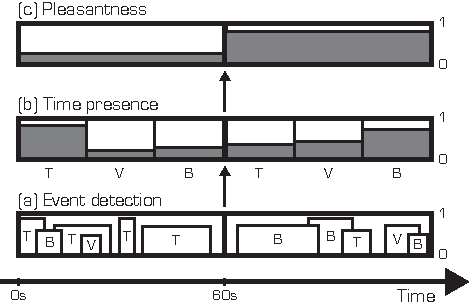
\includegraphics[width=.4\columnwidth]{figures/block} \\
\end{center}
\begin{itemize}
\item les qualifiants perceptifs de haut niveau comme l'agrément sont corrélés au temps de présence perçus des sources présentes dans la scène
\item prédiction de ces valeurs perceptives par des approches neuronales
\end{itemize}
\footfullcitenomarkleft{gontierActa}

\end{frame}

\begin{frame}{Projet de recherche avec le Conservatoire National de Musique et de Danse de Paris (CNSMDP)}
\begin{itemize}
\item Recherche par similarité dans des corpus de modes de jeux étendus
\item Confrontation d'un modèle computationnel de perception à des jugements experts
\item l'opérateur de diffusion d'ondelettes apporte d'excellents résultats
\end{itemize}
\begin{table}
\small
    \centering 
    
\begin{tabular}{c|ccccc}
 joint (1s) + lmnn & -lmnn & (25 ms) &  séparable & mfcc & \\
      \hline
 $96\% \pm 2$ & $93\% \pm 3$ & $91\% \pm 4$ & $91\% \pm 4$ & $82\% \pm 7$ & ($aP@5$)\\
\end{tabular}
\end{table}

\footfullcitenomarkleft{lostanlenJasmp}
\end{frame}


E

reproducibilité

donoho

protocoles expérimentaux assez canonique

explanes

extension de bande

demonstration






\begin{frame}{Approches étudiées}
\begin{center}
\includegraphics[width=.3\columnwidth]{figures/play} \\
\end{center}
\begin{description}
\item[$X$] plus de contrôle : données simulées
\item[$E$] plus de formalisation : dévelopement d'expLanes
\item[$Y$] plus de maîtrise : collaboration avec les communautés expertes
\end{description}
\end{frame}

\begin{frame}{Itemize}
\begin{itemize}
\item
\item
\item
\end{itemize}
\end{frame}
